\documentclass[sigconf,review,anonymous]{acmart}

% TODO copyright
\setcopyright{none}
% \setcopyright{acmcopyright}
% \copyrightyear{2018}
% \acmYear{2018}
% \acmDOI{XXXXXXX.XXXXXXX}

% TODO conference
% \acmConference[Conference acronym 'XX]{Make sure to enter the correct
%   conference title from your rights confirmation emai}{June 03--05,
%   2018}{Woodstock, NY}
% \acmPrice{15.00}
% \acmISBN{978-1-4503-XXXX-X/18/06}

%% Bibliography style
\bibliographystyle{ACM-Reference-Format}

%% macros with packages
% load packages
\usepackage{cite}
\usepackage{float}
\usepackage{amsmath,amssymb,amsfonts,amsthm}
\usepackage[ruled, vlined]{algorithm2e}
\usepackage{graphicx}
\usepackage{textcomp}
\usepackage{xcolor}
\usepackage{listings}
\usepackage{caption}
\usepackage{subcaption}
\usepackage{multirow}
\usepackage{booktabs}
\usepackage{makecell}
\usepackage{galois}
\usepackage{mathpartir}
\usepackage{bussproofs}
\usepackage{mathtools}
\usepackage{colortbl}
\usepackage{hhline}
\usepackage{stmaryrd}
\usepackage{microtype}
\usepackage{hyperref}
\usepackage{balance}

% basic
\newcommand{\inred}[1]{{\color{red}{#1}}}
\newcommand{\todo}{\inred{TODO}}
\newcommand{\name}[1]{\textsf{#1}}
\newcommand{\sname}[1]{\name{\small #1}}
\newcommand{\stextbf}[1]{\textbf{\small #1}}
\definecolor{dkgreen}{rgb}{0,0.5,0}
\definecolor{esvar}{HTML}{36702F}
\definecolor{esalg}{HTML}{376BA2}

% tools
\newcommand{\tool}{\sname{JSynView}}
\newcommand{\bigtool}{\name{JSynView}}
\newcommand{\esmeta}{\sname{ESMeta}}
\newcommand{\jiset}{\sname{JISET}}
\newcommand{\jest}{\sname{JEST}}
\newcommand{\jstar}{\sname{JSTAR}}
\newcommand{\asfsdf}{\textsc{Asf+Sdf}}

% ECMAScript Intermediate Representations (IRES)
\newcommand{\ires}{\text{IR}_\text{ES}}
\lstdefinestyle{ires}{
  frame=tb,
  aboveskip=3mm,
  belowskip=3mm,
  showstringspaces=false,
  columns=fixed,
  basicstyle={\footnotesize\ttfamily},
  numberstyle=\tiny\color{darkgray},
  numbers=none,
  numbersep=5pt,
  keywordstyle=\color{blue},
  comment=[l]{//},
  morecomment=[s]{/*}{*/},
  commentstyle=\color{dkgreen},
  stringstyle=\color{mauve},
  frame=single,
  breaklines=true,
  breakatwhitespace=true,
  tabsize=3,
}

% JavaScript code style
\lstdefinelanguage{JavaScript}{
  keywords={async, await, break, case, catch, class, const, continue, debugger,
    default, delete, do, else, enum, export, extends, false, finally, for,
    function, if, import, in, of, instanceof, new, null, return, super, switch, this,
    throw, true, try, typeof, let, var, void, while, with, yield},
  keywordstyle=\color{blue}\bfseries,
  ndkeywordstyle=\color{darkgray}\bfseries,
  identifierstyle=\color{black},
  numberstyle=\tiny\color{darkgray},
  numbers=none,
  numbersep=5pt,
  sensitive=false,
  comment=[l]{//},
  morecomment=[s]{/*}{*/},
  commentstyle=\color{dkgreen},
  stringstyle=\color{red}\ttfamily,
  morestring=[b]',
  morestring=[b]",
  morestring=[b]`
}
\lstdefinestyle{JS}{
  language=JavaScript,
  extendedchars=true,
  basicstyle=\footnotesize\ttfamily,
  showstringspaces=false,
  showspaces=false,
  tabsize=2,
  breaklines=true,
  showtabs=false,
  captionpos=b
}

% codes
\newcommand{\jscode}[1]{\text{\lstinline[style=JS,basicstyle=\small\ttfamily]!#1!}} 
\newcommand{\ircode}[1]{\text{\lstinline[style=ires,basicstyle=\small\ttfamily]!#1!}}
\newcommand{\code}[1]{{\small \texttt{#1}}}
\newcommand{\kwdef}{\code{def}}
\newcommand{\kweq}{\code{=}}
\newcommand{\kwret}{\code{ret}}
\newcommand{\kwif}{\code{if}}
\newcommand{\kwrl}{\code{(}}
\newcommand{\kwrr}{\code{)}}
\newcommand{\kwcl}{\code{\{}}
\newcommand{\kwcr}{\code{\}}}
\newcommand{\kwsl}{\code{[}}
\newcommand{\kwsr}{\code{]}}

% ECMAScript fonts
\newcommand{\esvar}[1]{{\color{esvar}{\textit{\small #1}}}}
\newcommand{\esalg}[1]{{\color{esalg}{\small #1}}}
\newcommand{\essyn}[1]{\textit{\small #1}}
\newcommand{\esval}[1]{\textbf{\small #1}}
\newcommand{\eswrd}[1]{{\small #1}}
\newcommand{\escall}[2]{#1\eswrd{(}#2\eswrd{)}}

% basic
\DeclareMathAlphabet{\mathpzc}{T1}{pzc}{m}{it}
\newcommand{\powerset}[1]{\mathcal{P}(#1)}
\newcommand{\abs}[1]{\widehat{#1}}
\newcommand{\finmap}{{\xrightarrow[]{\text{fin}}}}
\newcommand{\mapstos}{\;\dot{\mapsto}\;}
\newcommand{\Dom}{\sname{Dom}}
\DeclarePairedDelimiter{\norm}{\lvert}{\rvert} 

% notations
\newcommand{\progset}{\mathfrak{P}}
\newcommand{\prog}{P}
\newcommand{\getfunc}{\code{func}}
\newcommand{\getinst}{\code{inst}}
\newcommand{\getnext}{\code{next}}
\newcommand{\funcset}{\mathcal{F}}
\newcommand{\func}{f}
\newcommand{\labset}{\mathcal{L}}
\newcommand{\lab}{\mathpzc{l}}
\newcommand{\labdot}[1]{{{\bullet_{\lab_{#1}}}}}
\newcommand{\ilab}{\lab_\iota}
\newcommand{\labnext}{\sname{next}}
\newcommand{\op}{\sname{op}}
\newcommand{\ops}{\dot{\op}}
\newcommand{\instset}{\mathcal{I}}
\newcommand{\inst}{i}
\newcommand{\exprset}{\mathcal{E}}
\newcommand{\expr}{e}
\newcommand{\referset}{\mathcal{R}}
\newcommand{\refer}{r}
\newcommand{\varset}{\mathcal{X}}
\newcommand{\varx}{\code{x}}
\newcommand{\vart}{\code{t}}
\newcommand{\varf}{\code{f}}

% values
\newcommand{\valset}{\mathbb{V}}
\newcommand{\val}{v}
\newcommand{\pvalset}{\valset_\name{prim}}
\newcommand{\pval}{p}
\newcommand{\strset}{\valset_\name{str}}
\newcommand{\str}{s}
\newcommand{\boolset}{\valset_\name{bool}}
\newcommand{\bool}{b}
\newcommand{\intset}{\valset_\name{int}}
\newcommand{\true}{\code{\#t}}
\newcommand{\false}{\code{\#f}}

% JavaScript ASTs
\newcommand{\treeset}{\mathbb{T}}
\newcommand{\tree}{t}
\newcommand{\nodeset}{\Phi}
\newcommand{\node}{\phi}
\newcommand{\subtree}{\lhd}
\newcommand{\getsubs}{\sname{subs}}
\newcommand{\treetop}{\code{\#}}
\newcommand{\ty}{\tau}
\newcommand{\nt}{N}
\newcommand{\eval}{\code{eval}}

% states
\newcommand{\stset}{\mathbb{S}}
\newcommand{\st}{\sigma}
\newcommand{\initstset}{\stset^\name{init}}
\newcommand{\initst}{\st^\sname{init}}

% heaps
\newcommand{\heapset}{\mathbb{H}}
\newcommand{\heap}{h}

% contexts
\newcommand{\ctxtset}{\mathbb{C}}
\newcommand{\ctxts}{\overline{\ctxt}}
\newcommand{\postfix}{\ll}
\newcommand{\ctxt}{c}

% environments
\newcommand{\envset}{\mathbb{E}}
\newcommand{\env}{\rho}

% addresses
\newcommand{\addrset}{\mathbb{A}}
\newcommand{\addr}{a}

% objects
\newcommand{\objset}{\mathbb{O}}
\newcommand{\obj}{o}

% semantics
\newcommand{\sem}[1]{\llbracket{#1}\rrbracket}
\newcommand{\trans}{\leadsto}

% restricted semantics
\newcommand{\rsem}[1]{\sem{#1}_\textbf{R}}
\newcommand{\entrystset}{\stset^\name{entry}}
\newcommand{\entrylab}{\lab^\name{entry}}

% abstract semantics
\newcommand{\asem}[1]{\abs{\sem{#1}}}

% transformations
\newcommand{\transform}[1]{\textbf{T}[#1]}

% partial evaluation
\newcommand{\peval}[1]{\textbf{PE}[#1]}

% transfer function
\newcommand{\transfer}{F}
\newcommand{\atransfer}{\abs{\transfer}}

% abstract states
\newcommand{\aelemset}{\abs{\mathbb{D}}}
\newcommand{\aelem}{\abs{d}}
\newcommand{\entryaelem}{\aelem^\name{entry}}

% abstract calling contexts
\newcommand{\actxtset}{\abs{\ctxtset}}
\newcommand{\actxt}{\abs{\ctxt}}
\newcommand{\ascallset}{\abs{\ctxtset}_\name{s}}
\newcommand{\ascall}{\abs{\ctxt}_\name{s}}
\newcommand{\adcallset}{\abs{\ctxtset}_\name{d}}
\newcommand{\adcall}{\abs{\ctxt}_\name{d}}
\newcommand{\funcbot}{\bot_\funcset}
\newcommand{\functop}{\top_\funcset}

% function summaries
\newcommand{\funcsumset}{\abs{\funcset}}
\newcommand{\funcsum}{\abs{\func}}

% abstract environments
\newcommand{\aenvset}{\abs{\envset}}
\newcommand{\aenv}{\abs{\env}}
\newcommand{\afsenvset}{\aenvset_\name{fs}}
\newcommand{\afsenv}{\aenv_\name{fs}}

% abstract values
\newcommand{\avalset}{\abs{\valset}}
\newcommand{\aval}{\abs{\val}}
\newcommand{\valbot}{\bot_\valset}
\newcommand{\valtop}{\top_\valset}

% syntactic views
\newcommand{\atreeset}{\abs{\treeset}}
\newcommand{\atree}{\abs{\tree}}
\newcommand{\anodeset}{\abs{\nodeset}}
\newcommand{\anode}{\abs{\node}}
\newcommand{\asubtree}{\abs{\subtree}}
\newcommand{\targetfunc}{\func_{\atree}}
\newcommand{\agetsubs}{\abs{\getsubs}}
\newcommand{\svhole}[1]{\langle #1 \rangle}

% abstract operations
\newcommand{\join}{\sqcup}
\newcommand{\bigjoin}{\bigsqcup}
\newcommand{\order}{\sqsubseteq}
\newcommand{\revorder}{\sqsupseteq}

% least fixed point
\newcommand{\lfp}{\textbf{lfp}}

% concretization
\newcommand{\atreegamma}{\gamma_{\atree}}
\newcommand{\anodegamma}{\gamma_{\anode}}
\newcommand{\aelemgamma}{\gamma_{\aelem}}
\newcommand{\adcallgamma}{\gamma_{\adcall}}
\newcommand{\ascallgamma}{\gamma_{\ascall}}
\newcommand{\afsenvgamma}{\gamma_{\afsenv}}
\newcommand{\aenvgamma}{\gamma_{\aenv}}
\newcommand{\avalgamma}{\gamma_{\aval}}

% theorems
\newtheorem{theorem}{Theorem}

% theorems
\newtheorem{lemma}{Lemma}


%% start document
\begin{document}

%% Title information
\title[Deep Understanding of JavaScript Specification
through Syntactic Views]
{Deep Understanding of JavaScript Language Specification
through Syntactic Views}

% XXX
% \title[Understanding Behaviors of JavaScript Language Features
% via Automatic Specification Reduction with Syntactic Views]
% {Understanding Behaviors of JavaScript Language Features\\
% via Automatic Specification Reduction with Syntactic Views}

% XXX
% \title[Deep Understanding of JavaScript Semantics
% via Automatic Specification Reduction with Syntactic Views]
% {Deep Understanding of JavaScript Semantics\\
% via Automatic Specification Reduction with Syntactic Views}

% XXX
% \title[Reducing Language Specification and Conformance Tests
% with Syntactic Views for Better Understanding of JavaScript]
% {Reducing Language Specification and Conformance Tests\\
% with Syntactic Views for Better Understanding of JavaScript}

% \author{Seungmin An}
% \authornote{These authors contributed equally to this work.}
% \orcid{0000-0002-4281-9386}
% \affiliation{
%   \department{School of Computing}
%   \institution{KAIST}
%   \city{Daejeon}
%   \country{South Korea}
% }
% \email{h2oche@kaist.ac.kr}
% 
% \author{Jihee Park}
% \authornotemark[1]
% \orcid{0000-0001-6792-5161}
% \affiliation{
%   \department{School of Computing}
%   \institution{KAIST}
%   \city{Daejeon}
%   \country{South Korea}
% }
% \email{jiheepark@kaist.ac.kr}
% 
% \author{Jihyeok Park}
% \authornotemark[1]
% \orcid{0000-0001-8387-1984}
% \affiliation{
%   \institution{Oracle Labs}
%   \city{Brisbane}
%   \country{Australia}
% }
% \email{jihyeok.park@oracle.com}
% 
% \author{Sukyoung Ryu}
% \orcid{0000-0002-0019-9772}
% \affiliation{
%   \department{School of Computing}
%   \institution{KAIST}
%   \city{Daejeon}
%   \country{South Korea}
% }
% \email{sryu.cs@kaist.ac.kr}

\begin{abstract}\label{sec:abstract}
  JavaScript is a widely-used programming language in diverse fields.  However,
  despite its popularity, developers and even JavaScript experts often suffer
  from its highly dynamic and complex nature.  Thus, when they desire to
  understand the detailed semantics of JavaScript, they refer to ECMA-262, a
  standard JavaScript language specification written in English.  However, it is
  challenging to understand all the \textit{possible behaviors} of a single or
  combination of language features by only referring to the specification.
  Besides, even if developers recognize a possible behavior of a language
  feature, finding \textit{example programs} that trigger the behavior is also
  not trivial.

  To alleviate this problem, we present $\tool$, which automatically infers
  possible behaviors of JavaScript language features from ECMA-262 and finds
  corresponding example programs in Test262, an official JavaScript conformance
  test suite.  We first introduce \textit{syntactic views} to help users
  indicate which language features they want to understand by restricting
  program syntax with a type bound.  Then, our tool 1) soundly reduces the call
  graph of ECMA-262 with a given syntactic view to infer possible behaviors and
  2) searches concrete example programs in Test262 that trigger such behaviors
  using their pre-collected execution traces.  For evaluation of $\tool$, we
  used the latest ECMA-262 (ES12, 2021), including \inred{2,640} algorithms,
  with \inred{177} basic syntactic views.  As a result, our tool reduced ES12 to
  \inred{109.4} algorithms in \inred{0.8s} and found \inred{42.3} Test262
  programs for each algorithm in \inred{3.2s} on average.  Furthermore, we
  conducted \inred{three} case studies with advanced syntactic views to
  demonstrate the practicality of $\tool$.
\end{abstract}


% TODO 2012 ACM Computing Classification System (CSS) concepts
% \begin{CCSXML}
% <ccs2012>
%  <concept>
%   <concept_id>10010520.10010553.10010562</concept_id>
%   <concept_desc>Computer systems organization~Embedded systems</concept_desc>
%   <concept_significance>500</concept_significance>
%  </concept>
%  <concept>
%   <concept_id>10010520.10010575.10010755</concept_id>
%   <concept_desc>Computer systems organization~Redundancy</concept_desc>
%   <concept_significance>300</concept_significance>
%  </concept>
%  <concept>
%   <concept_id>10010520.10010553.10010554</concept_id>
%   <concept_desc>Computer systems organization~Robotics</concept_desc>
%   <concept_significance>100</concept_significance>
%  </concept>
%  <concept>
%   <concept_id>10003033.10003083.10003095</concept_id>
%   <concept_desc>Networks~Network reliability</concept_desc>
%   <concept_significance>100</concept_significance>
%  </concept>
% </ccs2012>
% \end{CCSXML}
%
% \ccsdesc[500]{Computer systems organization~Embedded systems}
% \ccsdesc[300]{Computer systems organization~Redundancy}
% \ccsdesc{Computer systems organization~Robotics}
% \ccsdesc[100]{Networks~Network reliability}

\keywords{JavaScript, syntactic view, partial evaluation}

\maketitle

%% body of the paper
\section{Introduction}\label{sec:intro}

In the beginning, JavaScript was a simple scripting language designed in a
ten-day hack. However, it has become a de facto Web standard and eventually
became one of the dominating programming languages in various fields. For
example, Node.js~\cite{nodejs} introduced full-stack JavaScript by supporting
server-side programming.  In addition, React Native~\cite{react-native} provides
a way to deploy JavaScript programs as mobile and desktop applications even
running on different platforms.  Furthermore, according to the annual report of
GitHub, JavaScript has consistently been the most popular programming language
based on the number of contributors to GitHub
projects.\footnote{\url{https://octoverse.github.com/}}

However, despite its popularity, developers and even JavaScript experts often
suffer from its highly dynamic nature.  It supports diverse language features
with complex semantics, including higher-order functions, mutable prototype
chains, dynamic code generation, and asynchronous functions.  For instance, even
addition and subtraction operations are not straightforward with complicated
implicit conversion rules.  Consider the following simple program:
\begin{center}
  \begin{tabular}{c}
    \begin{lstlisting}[style=JS]
'42' + 1 - 1 // result: 420
    \end{lstlisting}
  \end{tabular}
\end{center}
Surprisingly, it produces a number $\code{420}$ because the $\code{+}$
operator between string and number values denotes a string concatenation while
the $\code{-}$ operator between them denotes a numerical subtraction.  Such a
highly dynamic nature of JavaScript causes pain even to JavaScript experts in
understanding the language semantics.  For example, while V8 is the most
widely-used JavaScript engine developed by Google for Node.js and Chrome web
browsers, its semantic bugs have consistently been reported to its issue
tracker.\footnote{\url{https://bugs.chromium.org/p/v8}}

Therefore, when they desire to understand the detailed semantics of JavaScript,
they refer to ECMA-262, the standard JavaScript language specification written
in English.  It describes the syntax using a variant of the extended Backus–Naur
form and the semantics as abstract algorithms.  Each algorithm describes the
language semantics in with ordered and structured steps.  The Ecma Technical
Committee 39 (TC39) has officially maintained ECMA-262 as an open-source GitHub
project,\footnote{\url{https://github.com/tc39/ecma262}} and it annually updates
the specification with new language features to quickly adapt to the users'
demands.  Thus, JavaScript developers should read this specification if they
want to learn the detailed semantics of new language features introduced every
year.  Especially, developers of JavaScript tools (e.g.,
interpreters~\cite{v8, jscore, spidermonkey, graaljs},
transpilers~\cite{babel},
code analysis tools~\cite{safe, safe2, tajs, wala, jsai},
verification tools~\cite{javert, javert2, ad-safety, javanni},
symbolic execution engines~\cite{symbolic-js, sym-js, expo-se},
or concolic testing engines~\cite{jalangi, type-conc-test})
must carefully read the detailed semantics of all language features described in
the JavaScript language specification.

Unfortunately, it is still challenging to 1) understand all the \textit{possible
behaviors} of language features and 2) find \textit{example programs} that
trigger such behaviors by only referring to ECMA-262.

First, it is not an easy task to answer which behaviors are possible in each
language feature.  It often provides hidden implicit behaviors unusual in other
languages, such as implicit function calls, implicit property reads/writes, or
runtime exceptions under special conditions.  For example, we can call functions
even using the addition operation without any function application syntax.  If
we want to understand all possible behaviors of the addition operation, we need
to read \inred{109} algorithms reachable from its evaluation algorithm.
Besides, the problem becomes more complicated if we want to know possible
behaviors of a language feature used with specific types of values or other
language features.

Second, even if users realize its specific behavior, it is nontrivial to find
example programs that trigger the behavior.  For example, assume that we want to
find an example program having an addition operation that causes implicit
function calls.  Then, we should first grasp the condition when the addition
operation implicitly invokes functions and then find a JavaScript program that
satisfies the condition like this:
\begin{center}
  \begin{tabular}{c}
    \begin{lstlisting}[style=JS]
"a" + {toString: ()=>"b"} // result: "ab"
    \end{lstlisting}
  \end{tabular}
\end{center}
In this code, the left and right operands have different types $\code{String}$
and $\code{Object}$, respectively.  The addition between them causes an
implicit conversion of the object to a string value, and the function in the
$\code{toString}$ property is implicitly invoked during the conversion.

To alleviate this problem, this paper presents $\tool$ for the advanced
understanding of JavaScript language specification with \textit{syntactic
views}.  We introduce a \textit{syntactic view}, an extension of a JavaScript
abstract syntax tree (AST) consisting of both concrete and abstract nodes with
optional type bounds.  Users can freely construct syntactic views depending on
which combination of language features they want to understand; concrete nodes
denote the parts they want to understand, and abstract ones denote the parts
they do not.

For a given syntactic view, the tool performs reachability analysis to
automatically reduce the call graph of ECMA-262 with a given syntactic view to
soundly infer \textit{possible behaviors}.  Our key observation is that the
reachability of specific algorithms in the language specification implies
possible behaviors of language features.  For example, the \esalg{Call}
algorithm in ECMA-262 represents the invocation of functions.  Thus, if the
reduced call graph of ECMA-262 with a syntactic view for the addition operation
contains the \esalg{Call} algorithm, it might cause implicit function calls.

In addition, $\tool$ searches for \textit{example programs} that trigger
possible behaviors in a given program pool.  The tool first collects execution
traces of all the programs in the pool and builds a database only once at
initialization time.  Then, if a user selects an algorithm as the target
behavior with a syntactic view, $\tool$ utilizes the database to quickly search for
example programs in the pool that touches the selected algorithm in the
semantics of the given syntactic view.  For example, if we selects the
\esalg{Call} algorithm with a syntactic view for addition operation, the tool
automatically searches for example programs having an addition operation that
causes implicit function calls.

Our contributions are as follows:
\begin{itemize}
  \item We introduce a \textit{syntactic view}, an extension of a JavaScript
    abstract syntax tree (AST) consisting of both concrete and abstract nodes
    with optional type bounds, to help users indicate which language features
    they want to understand.

  \item We present an automatic way to 1) infer \textit{possible behaviors} of
    JavaScript language features using a reachability analysis in ECMA-262 and
    2) search \textit{example programs} that trigger such behaviors in a given
    program pool using their pre-collected execution traces.

  \item We actualize our techniques in $\tool$, evaluate its effectiveness using
    the latest ECMA-262 with \inred{177} basic syntactic views, and demonstrate
    its practicality with \inred{three} advanced syntactic views.
\end{itemize}

\section{Motivating Examples}\label{sec:motivation}

% \begin{figure}
%   \centering
%   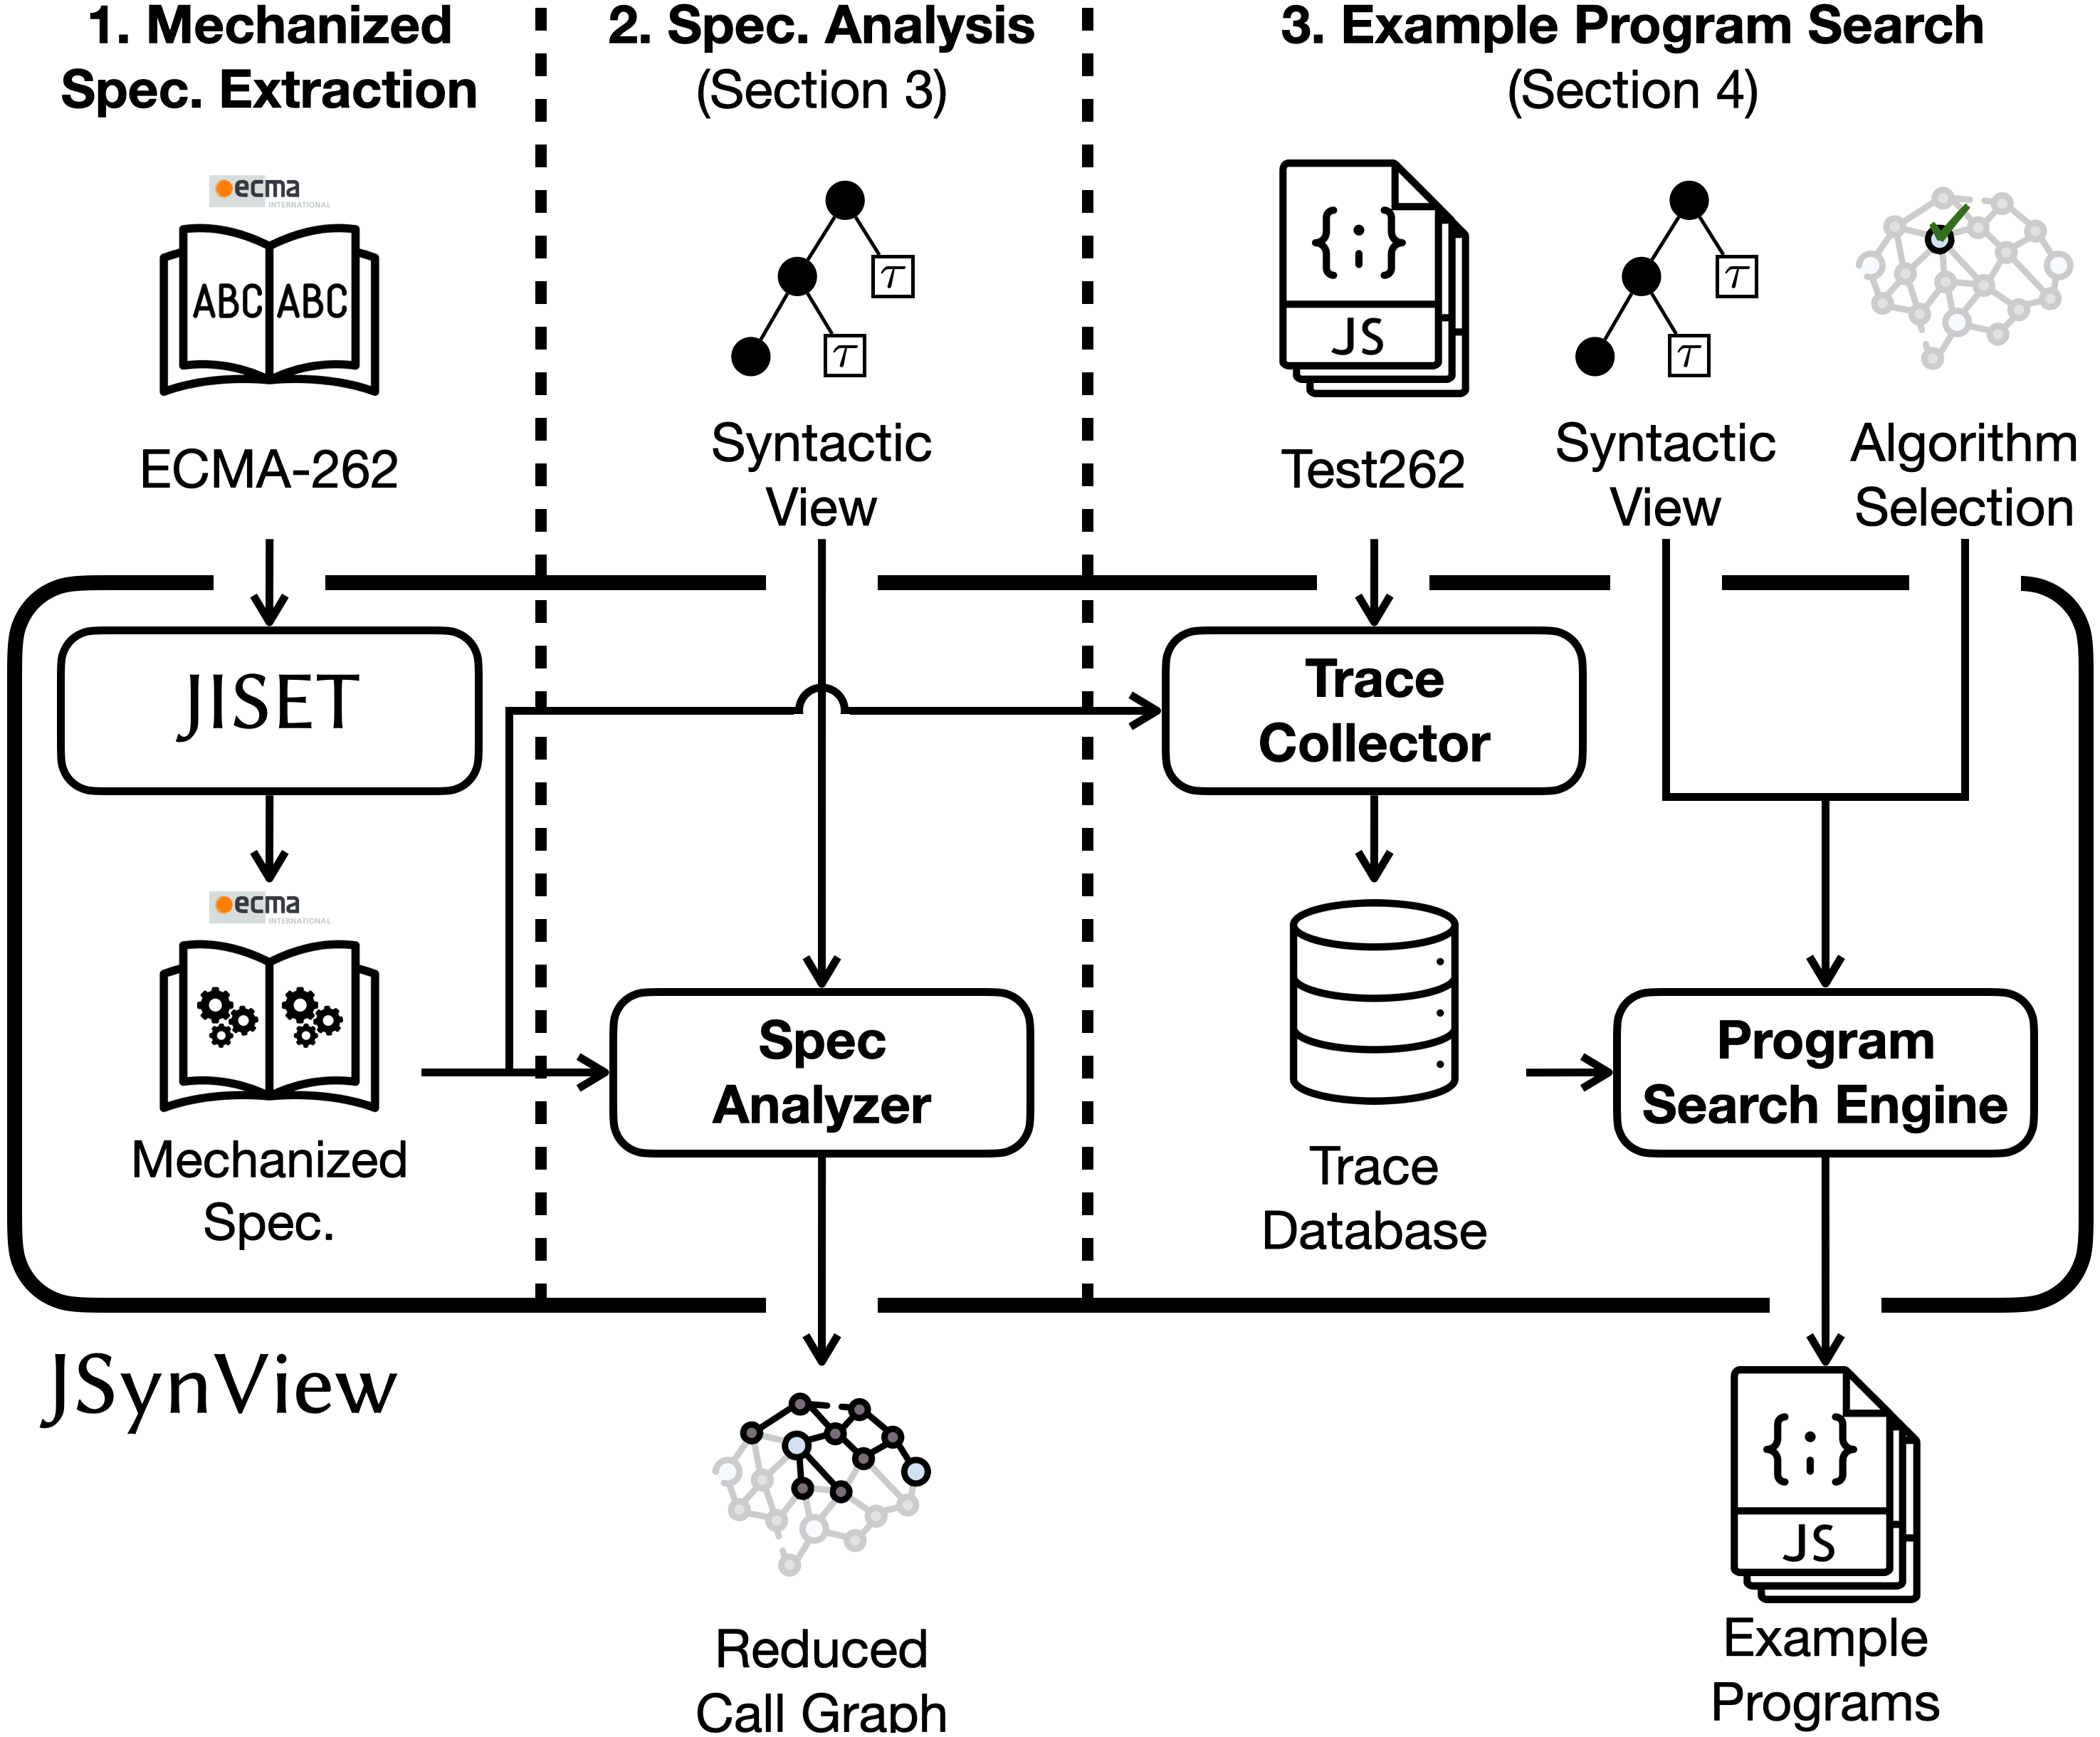
\includegraphics[width=\columnwidth]{img/overall.png}
%   \caption{The overall structure of $\tool$, a JavaScript interactive
%     specification supporting \textit{syntactic view selection} and
%   \textit{algorithm step selection}}
%   \label{fig:overall}
% \end{figure}
% 
% This section explains the overall structure of $\tool$ depicted in
% Figure~\ref{fig:overall}.
% 
% \todo

% It consists of four different modules: $\jiset$,
% \name{Step-by-Step Executor}, \name{Partial Evaluator}, and \name{Delta
% Debugger}. First, $\tool$ utilizes another tool called $\jiset$ to extract
% mechanized specification from ECMAScript.  Therefore, it is automatically
% synchronized with a given version of ECMAScript and deals with language
% semantics of the given specification.
% 
% \paragraph{Step-by-Step Execution}
% 
% dependent on a given version of ECMAScript.
% 
% extracts the JavaScript
% syntax and semantics using $\jiset$ and extracts specification types from
% ECMAScript.
% 
% \paragraph{Syntax and Semantics}
% 
% , 3) 
% 
% Our tool is a JavaScript interactive specification
% automatically synchronized with a given version of ECMAScript and supporting
% three different user interactions for better understanding of JavaScript
% language semantics. 
% 
% First, it supports \textit{step-by-step program
% execution} of a given JavaScript program with various debugging features
% 
% by strictly following the English
% sentences of the specification
% 
% by closely following the English
% sentences of the specification.
% 
% \textit{step-by-step
% execution} with various automatically synchronized with a given version of
% ECMAScript supporting k
% 
% 
% 
% which takes a specific version of ECMAScript and supports various user
% interactions for better understanding.
% automatically synchronized
% 
% depending on a given version of standard JavaScript specification, ECMAScript.
% It provides three interactions1) step-by-step execution, 2) partial
% evaluation with syntactic views, and 3) delta debugging with algorithm steps and
% JavaScript programs.
% 
% 
% official JavaScript
% dependent iwth 
% 
% takes a specific version of ECMAScript

\section{Syntactic Views}\label{sec:syn-view}

\todo

\section{Language Specification Reduction}\label{sec:spec-reduce}

\todo

\section{Conformance Test Reduction}\label{sec:test-reduce}

\todo

\section{Implementation}\label{sec:impl}

\todo

\begin{itemize}
  \item algorithm to find target syntactic view
  \item type annotation $\Rightarrow$ abstract value?
  \item context/loop-insensitive
  \item flow-sensitive
  \item abstract domain
    \begin{itemize}
      \item clo/cont - set
      \item comp - complex structure? for precision
      \item other - flat
      \item total - prod
    \end{itemize}
\end{itemize}

\section{Evaluation}\label{sec:eval}

\begin{itemize}
  \item \textbf{RQ1)} Can syntactic views express language features or their
    combinations developers desire to understand? (Section~\ref{eval-sview})
  \item \textbf{RQ2)} Does the reachability analysis soundly reduce the number
    of reachable algorithms in ECMA-262, and how many algorithms are reduced?
    (Section~\ref{eval-analysis})
  \item \textbf{RQ3)} How long does the program search engine take time to find
    out the target programs? (Section~\ref{eval-search})
  \item \textbf{RQ4)} Does $\tool$ enhance the understanding of possible
    behaviors of JavaScript language features? (Section~\ref{eval-study})
\end{itemize}

\todo

\subsection{Expressiveness of Syntactic Views}~\label{eval-sview}

frequently questionable features in blogs/stack overflow?
people's need?
syntactic view is general?

\todo

\subsection{Effectiveness of Reachability Analysis}~\label{eval-analysis}

\todo

\subsection{Performance of Program Search Engine}~\label{eval-search}

\todo

\subsection{Case Study: Advanced Understanding}~\label{eval-study}

\todo

\section{Related Work}\label{sec:related}

\begin{itemize}
  \item JavaScript specificaiton: ECMAScript (ES13, 2022)~\cite{es13}
  \item JavaScript tests: Test262~\cite{test262}
  \item JavaScript tools: engines~\cite{v8, jscore, chakra, spidermonkey},
    static analyzers~\cite{safe, safe2, tajs, wala, jsai},
    debugger~\cite{jsexplain}, verification tools~\cite{javert, javert2,
    ad-safety, javanni}, symbolic execution~\cite{symbolic-js, sym-js, expo-se},
    concolic testing~\cite{jalangi, type-conc-test}.
  \item Language Design Assistant (LDA)~\cite{lda, lisa, ipld, asf-sdf,
    meta-env, faustine}
  \item Domain Specific Language (DSL)~\cite{dsl-survey, dsl-survey2}
  \item Live Programming~\cite{omnicode, situ-vis, proj-box}
  \item JISET family: $\jiset$~\cite{jiset}, $\jest$~\cite{jest}, $\jstar$~\cite{jstar}.
  \item Partial Evaluation~\cite{peval, peval-survey}, Program
    Transformation~\cite{trans-ai}.
\end{itemize}

\todo

\section{Conclusion}\label{sec:conclusion}

\todo


%% Bibliography

%% the bibliography file.
\balance
\bibliography{ref}

%% Appendix
\appendix

\section{JavaScript Semantics Specialization with Syntactic Views}\label{sec:formal}

In this section, we introduce a JavaScript semantics specialization with
syntactic views.  We first introduce $\ires$ as a specification language to
describe JavaScript semantics. To provide options to select target semantics, we
also introduce syntactic views as an abstraction of JavaScript ASTs.  Then, we
define a JavaScript semantics specialization with syntactic views as a partial
evaluation of $\ires$ programs, which is a combination of static analysis and
program transformation. Finally, we prove the semantics preservation of the
partial evaluation.

\subsection{$\ires$: Intermediate Representations for ECMAScript}

We first introduce $\ires$, an \textbf{I}ntermediate \textbf{R}epresentations
for \textbf{E}CMA\textbf{S}cript, as a specification language for JavaScript to
describe JavaScript semantics. We define its abstract syntax, states, and
concrete semantics in the remainder of this section.

\subsubsection{Abstract Syntax}

\[
  \begin{array}{lr@{~}c@{~}c@{~}c@{~}l}
    \text{Programs} & \progset &\ni& \prog &=& (\initstset{\prog},
    \getfunc{\prog}, \getinst{\prog}, \getnext{\prog})\\

    \text{Functions} & \funcset &\ni& \func &::=&
    \kwdef \; \kwrl \varx^* \kwrr \; \lab\\

    \text{Variables} & \varset &\ni& \varx\\

    \text{Instructions} & \instset &\ni& \inst &::=&
    \refer \kweq \expr \mid
    \varx \kweq \kwcl \kwcr \mid
    \varx \kweq \expr \kwrl \expr^* \kwrr \mid \\&&&&&
    \kwif \; \expr \; \lab \; \lab \mid
    \kwret \; \expr\\

    \text{Labels} & \labset &\ni& \lab\\

    \text{Expressions} & \exprset &\ni& \expr &::=&
    \pval \mid
    \op \kwrl \expr^* \kwrr \mid
    \refer\\

    \text{References} & \referset &\ni& \refer &::=&
    \varx \mid \expr \kwsl \expr \kwsr\\
  \end{array}
\]

An $\ires$ program $\prog = (\initstset{\prog}, \getfunc{\prog},
\getinst{\prog}, \getnext{\prog}) \in \progset $ consists of initial states and
three mappings; $\getfunc{\prog}: \labset \rightarrow \funcset$ and
$\getinst{\prog}: \labset \rightarrow \instset$ map labels to their functions
and instructions, respectively, and $\getnext{\prog}: \labset \rightarrow
\labset$ maps labels to their next labels, where a label $\lab \in \labset$
denotes a program point.  A function $\func \in \funcset$ is defined with its
parameters and body label.  For presentation brevity, we assume that no global
or captured variables exist in this paper.  An instruction $\inst \in \instset$
is an assignment $\refer \kweq \expr$, an object allocation $\varx \kweq \kwcl
\kwcr$, a function call $\varx \kweq \expr \kwrl \expr^* \kwrr$, a branch $\kwif
\; \expr \; \lab \; \lab$, or a return instruction $\kwret \; \expr$.  An
invocation of an abstract algorithm in ECMAScript is compiled to a function call
instruction with a new temporary variable.  We represent loops using branch
instructions with cyclic pointing of labels in $\getnext{\prog}$.  An expression
is a primitive value $\pval$, an operation $\op \kwrl \expr^* \kwrr$, or a
reference $\refer$.  A reference is a variable $\varx$ or an object field $\expr
\kwsl \expr \kwsr$.  We write $\expr.\varf$ to briefly represent $\expr \kwsl
\code{"f"} \kwsr$.


\subsubsection{States}

\[
  \begin{array}{lr@{~}c@{~}l@{~}c@{~}l}
    \text{States} & \st &\in& \stset &=&
    \labset \times \ctxtset^* \times \heapset \times \envset\\

    \text{Calling Contexts} & \ctxt &\in& \ctxtset &=&
    \labset \times \envset \times \varset\\

    \text{Heaps} & \heap &\in& \heapset &=&
    \addrset \finmap \objset\\

    \text{Objects} & \obj &\in& \objset &=&
    \strset \finmap \valset\\

    \text{Environments} & \env &\in& \envset &=&
    \varset \finmap \valset\\

    \text{Values} & \val &\in& \valset &=&
    \pvalset \uplus \addrset \uplus \treeset \uplus \funcset\\

    \text{Primitive Values} & \pval &\in& \pvalset &=&
    \boolset \uplus \intset \uplus \strset \uplus \cdots\\

    \text{JavaScript ASTs} & \tree &\in& \treeset\\
  \end{array}
\]

States $\stset$ consist of labels $\labset$, calling context stacks
$\ctxtset^*$, heaps $\heapset$, and environments $\envset$.  A calling context
$\ctxt \in \ctxtset$ consists of a label denoting the return point, a caller's
environment, and a return variable.  A heap $\heap \in \heapset$ is a finite
mapping from addresses to objects, and an object $\obj \in \objset$ is a finite
mappings from strings to values.  Each object allocation $\kwcl \kwcr$ creates a
unique address $\addr \in \addrset$ different from existing addresses.  An
environment $\env \in \envset$ is a finite mapping from variables to values. A
value $\val \in \valset$ is a primitive value $\pval \in \pvalset$ (e.g., a
boolean value $\bool \in \boolset$, an integer $k \in \intset$, or a string
$\str \in \strset$), an address $\addr \in \addrset$, a JavaScript AST $\tree
\in \treeset$, or a function $f \in \funcset$.

$\ires$ is a specification language for JavaScript that treats JavaScript ASTs
as its values. To handle JavaScript ASTs in $\ires$, we define them with tree
nodes $\nodeset$ as follows:
\[
  \begin{array}{l@{~}c@{~}l@{~}c@{~}l}
    \treeset &\ni& \tree &::=& \nt_k \langle \node^* \rangle\\
    \nodeset &\ni& \node &::=& \str \mid \tree\\
  \end{array}
\]
A JavaScript AST $\nt_k \langle \node_1, \cdots, \node_n \rangle$ denotes $k$-th
alternative in the syntactic production of nonterminal symbol $\nt$ with
multiple tree nodes $\node_1, \cdots, \node_n$.  A tree node is a string for a
terminal symbol or another tree for a nonterminal symbol. We define several
notations to easily deal with JavaScript ASTs.  The notation $\nt_k.\eval$ denotes
an \esalg{Evaluation} function of $k$-th alternative in the production $\nt$.
Similarly, the notation $\tree.\eval$ denotes the \esalg{Evaluation} function of
the AST $\tree$, and it is same with $\nt_k.\eval$ when $\tree = \nt_k \langle
\cdots \rangle$. The \esalg{Evaluation} of each AST takes the AST itself and its
tree nodes that are nonterminals as arguments.  The notation $\getsubs(\tree)$
denotes tree nodes that are subtrees of $\tree$.  For example,
Figure~\ref{fig:coalesce-prod} shows a syntactic production for coalesce
expressions.  Consider the following JavaScript coalesce expression:
\begin{lstlisting}[style=JS]
                    42 ?? true
\end{lstlisting}
Then, the following AST is produced as its parsing result:
\[
  \begin{array}{lcl}
    \tree_0 &=&
    \essyn{CoalesceExpression}_0 \langle \tree_1, \code{"??"}, \tree_2 \rangle\\

    \tree_1 &=&
    \essyn{CoalesceExpressionHead}_1 \langle \tree_3 \rangle\\

    \tree_2 &=&
    \essyn{BitwiseORExpression}_0 \langle \cdots \rangle\\

    \tree_3 &=&
    \essyn{BitwiseORExpression}_0 \langle \cdots \rangle\\
  \end{array}
\]
\begin{figure}[H]
  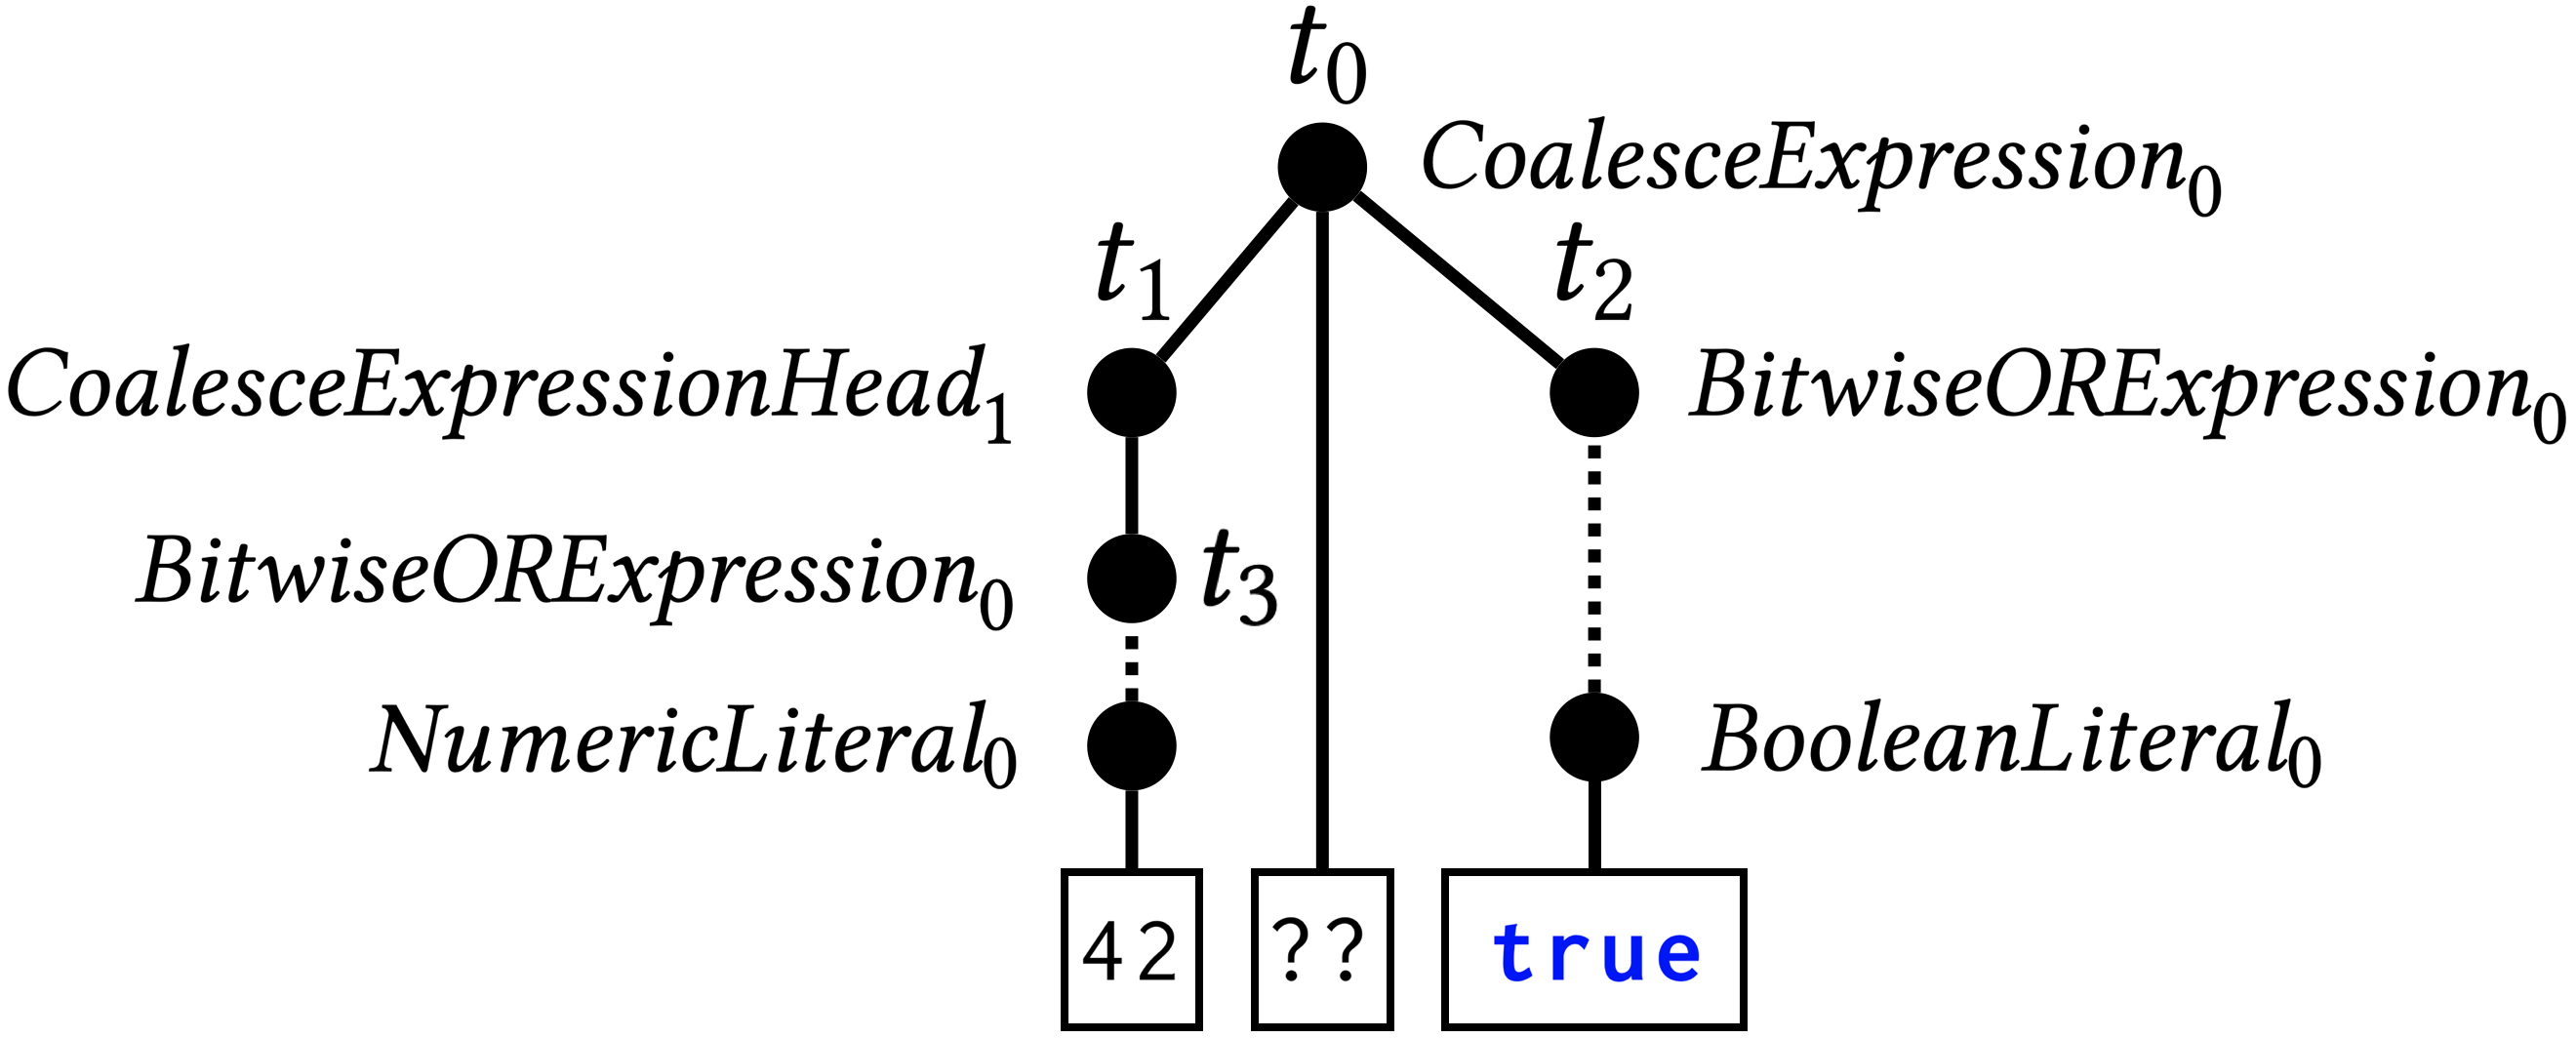
\includegraphics[width=.8\columnwidth]{img/ast-example.png}
\end{figure}
\noindent Its \esalg{Evaluation} function $\essyn{CoalesceExpression}_0.\eval$
takes three subtrees as arguments annotated by $\tree_0$, $\tree_1$, and
$\tree_2$ in the figure. The ASTs $\tree_0$, $\tree_1$, $\tree_2$, and $\tree_3$
are subtrees of $\tree_0$ (i.e., $\tree_0 \subtree \tree_0, \cdots, \tree_3
\subtree \tree_0$), and $\getsubs(\tree_0) = [\tree_1, \tree_2] \wedge
\getsubs(\tree_1) = [\tree_3]$.


\begin{figure}
  \centering
  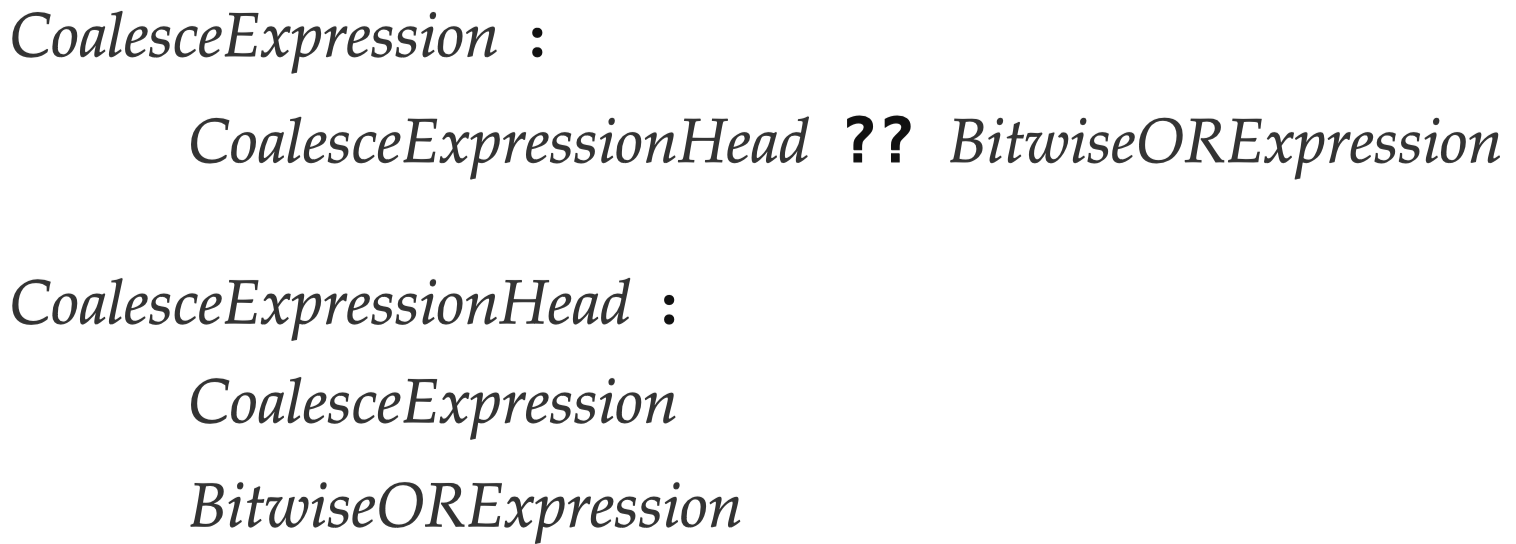
\includegraphics[width=.8\columnwidth]{img/coalesce-prod.png}
  \caption{A JavaScript syntactic production for coalesce expressions}
  \label{fig:coalesce-prod}
\end{figure}




\subsubsection{Concrete Semantics}

The concrete semantics $\sem{\prog}$ of an $\ires$ program $\prog$ is defined as
follows:
\[
  \sem{\prog} = \{ \st \in \stset \mid \exists \initst \in \initstset{\prog}. \;
  \initst \trans{\prog}^* \st \}
\]
where $\trans{\prog}^*$ denotes one or more repetition of $\trans{\prog}$, and
$\st \trans{\prog} \st'$ if and only if $\st = (\lab, \_, \_, \_)$ and
$\sem{\getinst{\prog}(\lab)}(\st) = \st'$. Another way to represent the concrete
semantics is to define a transfer function $\transfer: \powerset{\stset}
\rightarrow \powerset{\stset}$:
\[
  \sem{\prog} = \lim_{n \rightarrow \infty}\transfer^n(\initstset{\prog})
\]
where
\begin{equation}\label{eqn:transfer}
  \transfer(S) = \{ \st' \in \stset \mid \exists \st \in S. \; \st \trans{\prog}
  \st' \}
\end{equation}
Now, we define the denotational semantics of expressions, instructions, and
functions.

\paragraph{Expressions} We define the denotational semantics of expressions with
the following form:
\[
  \framebox{$\sem{\expr}: \stset \rightarrow \valset$}
\]
For each expression $\expr \in \exprset$, its semantics $\sem{\expr}$ takes a
state and returns a value as the result of expression. We define four different
cases in the semantics of expressions as
follows:
\begin{itemize}
  \item \underline{Primitive Values}:
    \[
      \sem{\pval}(\st) = \pval
    \]

  \item \underline{Operations}:
    \[
      \sem{\op \kwrl \expr_1, \cdots, \expr_n \kwrr}(\st) =
      \op(\val_1, \cdots, \val_n)
    \]
    where $\forall 1 \leq j \leq n. \; \sem{\expr_k}(\st) = \val_j$

  \item \underline{Variable Lookups}:
    \[
      \sem{\varx}(\st) = \env(\varx)
    \]
    where $\st = (\_, \_, \_, \env)$

  \item \underline{Field Lookups}:
    \[
      \sem{\expr_0 \kwsl \expr_1 \kwsr}(\st) = \val
    \]
    where
    \[
      \begin{array}{l@{~}c@{~}ll}
        \val_0 &=& \sem{\expr_0}(\st) &\wedge\\
        \val_1 &=& \sem{\expr_1}(\st) &\wedge\\
        \st &=& (\_, \_, \heap, \_) &\wedge\\
        \val &=& \left\{
          \begin{array}{ll}
            \heap(\addr)(\str)
            & \text{if} \; \val_0 = \addr \wedge \val_1 = \str\\

            \tree_j
            & \text{if} \; \val_0 = \nt_k \langle \tree_1, \cdots, \tree_n
            \rangle \wedge \val_1 = j\\

            \nt_k.\eval
            & \text{if} \; \val_0 = \nt_k \langle \tree_1, \cdots, \tree_n
            \rangle \wedge \val_1 = \code{"eval"}\\
          \end{array}
        \right.\\
      \end{array}
    \]
\end{itemize}

\paragraph{Instructions} We define the denotational semantics of instructions
with the following form:
\[
  \framebox{$\sem{\inst}: \stset \rightarrow \stset$}
\]
For each instruction $\inst \in \instset$, its semantics $\sem{\inst}$ takes a
state and returns an updated state. We define six different cases in the
semantics of instructions as follows:

\begin{itemize}
  \item \underline{Variable Assignments}:
    \[
      \sem{\varx \kweq \expr}(\st) =
      (\getnext{\prog}(\lab), \ctxts, \heap, \env[\varx \mapsto \val])
    \]
    where $\sem{\expr}(\st) = ((\lab, \ctxts, \heap, \env), \val)$

  \item \underline{Field Assignments}:
    \[
      \sem{\expr_0 \kwsl \expr_1 \kwsr \kweq \expr_2}(\st) =
      (\getnext{\prog}(\lab), \ctxts, \heap[\addr \mapsto \obj'], \env)
    \]
    where
    \[
      \begin{array}{l@{~}c@{~}ll}
        \sem{\expr_0}(\st) &=& (\st', \addr) &\wedge\\
        \sem{\expr_1}(\st') &=& (\st'', \str) &\wedge\\
        \sem{\expr_2}(\st'') &=& ((\lab, \ctxts, \heap, \env), \val) &\wedge\\
        \obj &=& \heap(\addr) &\wedge\\
        \obj' &=& \obj[\str \mapsto \val]\\
      \end{array}
    \]

  \item \underline{Object Allocations}:
    \[
      \sem{\varx \kweq \kwcl \kwcr}(\st) =
      (\lab, \ctxts, \heap[\addr \mapsto \epsilon], \env[\varx \mapsto
      \addr])
    \]
    where $\st = (\lab, \ctxts, \heap, \env) \wedge \addr \not\in
    \text{Domain}(\heap)$

  \item \underline{Function Calls}:
    \[
      \sem{\varx \kweq \expr \kwrl \expr_1 \cdots \expr_n \kwrr}(\st) =
      (\lab_\varf, \ctxt :: \ctxts, \heap, \env')
    \]
    where
    \[
      \begin{array}{l@{~}c@{~}ll}
        \sem{\expr}(\st) &=& (\st_0, \kwdef \; \kwrl \varx_1, \cdots, \varx_n
        \kwrr \; \lab_\varf) &\wedge\\
        \sem{\expr_j}(\st_{j-1}) &=& (\st_j, \val_j) \;
        [\forall 1 \leq j \leq n] &\wedge\\
        \st_n &=& (\lab, \ctxts, \heap, \env) &\wedge\\
        \env' &=& [\varx_1 \mapsto \val_1, \cdots, \varx_n \mapsto \val_n]
        &\wedge\\
        \ctxt &=& (\getnext{\prog}(\lab), \env, \varx)\\
      \end{array}
    \]

  \item \underline{Branches}:
    \[
      \sem{\kwif \; \expr \; \lab_\vart \; \lab_\varf}(\st) =
      \left\{
        \begin{array}{ll}
          (\lab_\vart, \ctxts, \heap, \env) & \text{if} \; \val = \true\\
          (\lab_\varf, \ctxts, \heap, \env) & \text{if} \; \val = \false\\
        \end{array}
      \right.
    \]
    where $\sem{\expr}(\st) = ((\lab, \ctxts, \heap, \env), \val)$

  \item \underline{Returns}:
    \[
      \sem{\kwret \; \expr}(\st) = (\lab, \ctxts, \heap, \env[\varx \mapsto
      \val])
    \]
    where $\sem{\expr}(\st) = ((\_, (\lab, \env, \varx) :: \ctxts, \heap, \_),
    \val)$
\end{itemize}


\subsection{Syntactic Views}

A syntactic view $\atree \in \atreeset$ is an abstract JavaScript AST with
abstract tree nodes $\anodeset$:
\[
  \begin{array}{l@{~}c@{~}l@{~}c@{~}l}
    \atreeset &\ni& \atree &::=& \nt_k \langle \anode^* \rangle \mid \nt\\
    \anodeset &\ni& \anode &::=& \str \mid \atree\\
  \end{array}
\]
where $\nt$ denotes all ASTs whose nonterminal symbol $\nt$. We define the
concretization of abstract trees $\atreegamma: \atreeset \rightarrow
\powerset{\treeset}$ and that of abstract nodes $\anodegamma: \anodeset
\rightarrow \powerset{\nodeset}$ as follows:
\[
  \begin{array}{lcl}
    \atreegamma(\nt_k \langle \anode_1, \cdots, \anode_n \rangle) &=&
    \{ \nt_k \langle \node_1, \cdots, \node_n \rangle \mid \node_j \in
    \anodegamma(\anode_j) \}\\

    \atreegamma(\nt) &=&
    \{ \tree \in \treeset \mid \tree = \nt_k \langle \cdots \rangle \}\\

    \anodegamma(\str) &=& \{ \str \}\\

    \anodegamma(\atree) &=& \atreegamma(\atree)\\
  \end{array}
\]
% \[
%   \begin{array}{lcl}
%     \anode \order \anode' &\Leftrightarrow& \left\{
%       \begin{array}{ll}
%         \anode = \anode' &\vee\\
% 
%         \anode' = \nt &\vee\\
% 
%         (\anode = \atree \wedge \anode' = \atree' \wedge \atree \order
%         \atree')\\
%       \end{array}
%     \right.\\
% 
%     \atree \order \atree' &\Leftrightarrow& \left\{
%       \begin{array}{ll}
%         \atree = \atree' &\vee\\
% 
%         \atree' = \treetop &\vee\\
% 
%         \begin{array}{@{}l@{}}
%           \atree = \nt_k \langle \atree_1, \cdots, \atree_n \rangle \wedge
%           \atree' = \nt_k \langle \atree'_1, \cdots, \atree'_n \rangle \wedge\\
%           \forall j. \; \tree_j \order \tree'_j\\
%         \end{array}\\
%       \end{array}
%     \right.\\
% 
%     \atree \join \atree' &=& \left\{
%       \begin{array}{ll}
%         \atree' & \text{if} \; \atree \order \atree'\\
% 
%         \atree & \text{if} \; \atree \revorder \atree'\\
% 
%         \nt_k \langle \atree''_1, \cdots, \atree''_n \rangle &
%         \text{if} \; \atree = \nt_k \langle \atree_1, \cdots, \atree_n \rangle
%         \wedge\\&
%         \phantom{\text{if} \;} \atree = \nt_k \langle \atree_1, \cdots, \atree_n
%         \rangle \wedge\\&
%         \phantom{\text{if} \;} \forall j. \; \atree''_j = \atree_j
%         \join \atree'_j\\
%         \treetop & \text{otherwise}\\
%       \end{array}
%     \right.\\
%   \end{array}
% \]
Moreover, we define abstract subtree relation $\asubtree \subseteq \atreeset
\times \treeset$:
\[
  \atree \; \asubtree \; \tree' \iff \exists \tree \in \atreegamma(\atree). \;
  \tree \subtree \tree'
\]
to filter out JavaScript programs not related to a given syntactic view.
Similar to $\getsubs(\tree)$, an abstract helper function $\agetsubs(\atree)$
denotes abstract tree nodes that are syntactic views when $\atree = \nt_k
\langle \cdots \rangle$.



\subsection{Partial Evaluation}

We define a \textit{partial evaluation} $\peval{\prog}: \atreeset \rightarrow
\progset$ of $\ires$ programs to specialize JavaScript semantics with a given
syntactic view:
\[
  \peval{\prog}(\atree) = \transform{\prog} \circ \asem{\prog} (\atree)
\]
It takes a syntactic view $\atree \in \atreeset$ to restrict arguments of the
corresponding \esalg{Evaluation} function. Then, it performs a static analysis
$\asem{\prog}$ of a given program $\prog$ with the syntactic view $\atree$, and
transforms the program to a specialized program using $\transform{\prog}$ with
the analysis result $\asem{\prog}(\atree)$.  Since the \esalg{Evaluation} of
$\nt$ might one or more $\ires$ functions, we only define the partial evaluation
when $\atree = \nt_k \langle \cdots \rangle$.  Now, we define the static
analysis and program transformation of $\ires$ programs and prove the semantics
preservation of the partial evaluation consisting of them.


\subsubsection{Static Analysis}

The static analysis $\asem{\prog}(\atree)$ performs an abstract
interpretation~\cite{ai1977, ai1992} to abstract concrete semantics under the
given given syntactic view $\atree$.  We first define abstract domains of
states, call edges, environments, and values as follows:
\begin{itemize}
  \item \underline{Abstract States}: $\aelemset$
    \[
      \begin{array}{lcl}
        \aelemset &=& \adcallset \times \ascallset \times \afsenvset\\

        \aelemgamma &:& \atreeset \rightarrow \aelemset \rightarrow
        \powerset{\stset}\\

        \aelemgamma(\atree)(\aelem) &=&
        (\adcallgamma(\atree)(\adcall) \setminus C) \uplus
        (C \cap \afsenvgamma(\afsenv))\\
        \multicolumn{3}{r}{\text{where} \; C = \ascallgamma(\atree)(\ascall)}\\

        \aelem \order \aelem' &\Leftrightarrow&
        \adcall \order \adcall' \wedge
        \ascall \order \ascall' \wedge
        \afsenv \order \afsenv'\\

        \aelem \join \aelem' &=&
        (\adcall \join \adcall', \ascall \join \ascall', \afsenv \join \afsenv')\\
      \end{array}
    \]
    where $\atree = \nt_k \langle \cdots \rangle$, $\aelem = (\adcall, \ascall,
    \afsenv)$ and $\aelem' = (\adcall', \ascall', \afsenv')$

  \item \underline{Dynamic Call Sets}: $\adcallset$
    \[
      \begin{array}{lcl}
        \adcallset &=& \powerset{\labset}\\

        \adcallgamma &:& \atreeset \rightarrow \adcallset \rightarrow
        \powerset{\stset}\\

        \adcallgamma(\atree)(\adcall) &=& \{ \st \in \stset \mid
          \st = (\lab, [\ctxt_1, \cdots, \ctxt_n], \_, \_) \wedge\\&&

          \phantom{\{ \st \in \stset \mid}
          \exists 1 \leq j \leq n. \; \ctxt_j = (\lab_j, \_, \_) \wedge\\&&

          \phantom{\{ \st \in \stset \mid}
          \lab_j \in \adcall
        \}\\

        \adcall \order \adcall' &\Leftrightarrow&
        \adcall \subseteq \adcall\\

        \adcall \join \adcall' &=&
        \adcall \cup \adcall\\
      \end{array}
    \]
    where $\atree = \nt_k \langle \cdots \rangle$

  \item \underline{Static Call Sets}: $\ascallset$
    \[
      \begin{array}{lcl}
        \ascallset &=& \powerset{\labset \times \funcset}\\

        \ascallgamma &:& \atreeset \rightarrow \ascallset \rightarrow
        \powerset{\stset}\\

        \ascallgamma(\atree)(\ascall) &=& \{ \st \in \stset \mid
          \st = (\lab_0, [\ctxt_1, \cdots, \ctxt_n], \_, \_) \wedge\\&&

          \phantom{\{ \st \in \stset \mid}
          \forall 1 \leq j \leq n. \; \ctxt_j = (\lab_j, \_, \_) \wedge\\&&

          \phantom{\{ \st \in \stset \mid}
          \exists 0 \leq m \leq n. \; \getfunc{\prog}(\lab_m) = \nt_k.\eval
          \wedge\\&&

          \phantom{\{ \st \in \stset \mid}
          \forall 1 \leq j \leq m. \; (\lab_j, \getfunc{\prog}{\lab_{j-1}}) \in
          \ascall
        \}\\

        \ascall \order \ascall' &\Leftrightarrow& \ascall \subseteq \ascall\\

        \ascall \join \ascall' &=& \ascall \cup \ascall'\\
      \end{array}
    \]
    where $\atree = \nt_k \langle \cdots \rangle$

  \item \underline{Flow-Sensitive Abstract Environments}: $\afsenvset$
    \[
      \begin{array}{lcl}
        \afsenvset &=& \labset \rightarrow \aenvset\\

        \afsenvgamma &:& \afsenvset \rightarrow \powerset{\stset}\\

        \afsenvgamma(\afsenv) &=& \{ \st \in \stset \mid
          \st = (\lab, \_, \_, \_) \wedge \st \in \aenvgamma(\afsenv(\lab))
        \}\\

        \afsenv \order \afsenv' &\Leftrightarrow&
        \forall \lab \in \labset. \; \afsenv(\lab) \order \afsenv'(\lab)\\

        \afsenv \join \afsenv' &=&
        \lambda \lab \in \labset. \; \afsenv(\lab) \join \afsenv'(\lab)\\
      \end{array}
    \]

  \item \underline{Abstract Environments}: $\aenvset$
    \[
      \begin{array}{lcl}
        \aenvset &=& \varset \rightarrow \aenvset\\

        \aenvgamma &:& \aenvset \rightarrow \powerset{\stset}\\

        \aenvgamma(\aenv) &=& \{ \st \in \stset \mid
          \forall \varx \in \varset. \;
          \sem{\varx}(\st) \in \avalgamma(\aenv(\varx))
        \}\\

        \aenv \order \aenv' &\Leftrightarrow&
        \forall \varx \in \varset. \;
        \aenv(\varx) \order \aenv'(\varx)\\

        \aenv \join \aenv' &=&
        \lambda \varx \in \varset. \;
        \aenv(\varx) \join \aenv'(\varx)\\
      \end{array}
    \]

  \item \underline{Abstract Values}: $\avalset$
    \[
      \begin{array}{lcl}
        \avalset &=& \valset \uplus \atreeset \uplus \{ \top, \bot,  \}\\

        \avalgamma &:& \avalset \rightarrow \powerset{\valset}\\

        \avalgamma(\aval) &=& \left\{
          \begin{array}{ll}
            \{ \val \} & \text{if} \; \aval = \val\\
            \atreegamma(\atree) & \text{if} \; \aval = \atree\\
            \valset & \text{if} \; \aval = \top\\
            \varnothing & \text{if} \; \aval = \bot\\
          \end{array}
        \right.\\

        \aval \order \aval' &\Leftrightarrow& \left\{
          \begin{array}{ll}
            \aval = \bot \vee \aval' = \top \vee \aval = \aval' & \vee\\
            \aval = \atree \wedge \aval' = \atree' \wedge
            \atree \order \atree' &\vee\\
            \aval = \tree \wedge \aval' = \atree' \wedge \tree \in
            \atreegamma(\atree')\\
          \end{array}
        \right.\\

        \aval \join \aval' &=& \left\{
          \begin{array}{ll}
            \aval' & \text{if} \; \aval \order \aval'\\
            \aval & \text{if} \; \aval \revorder \aval'\\
            \top & \text{otherwise}\\
          \end{array}
        \right.\\
      \end{array}
    \]
\end{itemize}

An abstract state $\aelem \in \aelemset$ is a triple of a dynamic call set, a
static call set, and a flow-sensitive abstract environment.  A dynamic call set
$\adcall \in \adcallset$ is a set of call labels representing function calls
with multiple functions or no static arguments. A static call set $\ascall \in
\ascallset$ is a set of possible static call edges from labels to function, and
it represent a set of \textit{static calling contexts}
$\ascallgamma(\ascall)(\atree)$ with a given syntactic view $\atree$ to
determine the scope of program transformations.  To more precisely in the static
calling contexts, we define a flow-sensitive abstract environment $\afsenv \in
\afsenvset$. It is a mapping from labels to abstract environments to represents
the shape of environments in each label. An abstract environment $\aenv \in
\aenvset$ is a mapping from variables to abstract values to describe values
stored in variables. An abstract value $\aval \in \avalset$ is a static value
$\val$, a syntactic view $\atree$, a dynamic value $\top$, or nothing $\bot$.
Now, we define abstract semantics of expressions, instructions, and programs.

\paragraph{Expressions} We first define abstract semantics of expressions as
follows:
\[
  \framebox{$\asem{\expr}: \aenvset \rightarrow \avalset$}
\]
\begin{itemize}
  \item \underline{Primitive Values}:
    \[
      \asem{\pval}(\aenv) = \pval
    \]
  \item \underline{Operations}:
    \[
      \asem{\op \kwrl \expr_1, \cdots, \expr_n \kwrr}(\aenv) = \aval
    \]
    where
    \[
      \begin{array}{l@{~}c@{~}l@{~}l}
        \asem{\expr_j}(\aenv) &=& \aval_j \; [\forall 1 \leq j \leq n]
        &\wedge\\
        \aval &=& \left\{
          \begin{array}{ll}
            \bot & \text{if} \; \exists j. \; \aval_j = \bot\\

            \op(\val_1, \cdots, \val_n) &
            \text{if} \; \forall j. \; \aval_j = \val_j\\

            \top & \text{otherwise}\\
          \end{array}
        \right.\\
      \end{array}
    \]
  \item \underline{Variable Lookups}:
    \[
      \asem{\varx}(\aenv) = \aenv(\varx)
    \]
  \item \underline{Field Lookups}:
    \[
      \asem{\expr_0 \kwsl \expr_1 \kwsr}(\aenv) = \aval
    \]
    where
    \[
      \begin{array}{lcl}
        \asem{\expr_0}(\aenv) &=& \aval_0\\
        \asem{\expr_1}(\aenv) &=& \aval_1\\
        \aval &=& \left\{
          \begin{array}{ll}
            \atree_j & \text{if} \;
            \aval_0 = \nt_k \langle \atree_1, \cdots, \atree_n \rangle \wedge
            \aval_1 = j\\

            \nt_k.\eval & \text{if} \;
            \aval_0 = \nt_k \langle \cdots \rangle \wedge
            \aval_1 = \code{"eval"}\\

            \top & \text{otherwise}\\
          \end{array}
        \right.\\
      \end{array}
    \]
\end{itemize}

\paragraph{Instructions} Then, we define the abstract semantics of instructions
as follows:
\[
  \framebox{$\asem{\inst}: \labset \times \aelemset \rightarrow \aelemset$}
\]
\begin{itemize}
  \item \underline{Variable Assignments}:
    \[
      \asem{\varx \kweq \expr}(\lab, \aelem) =
      (\adcall, \ascall, [\getnext{\prog}(\lab) \mapsto \aenv[\varx
      \mapsto \aval]])
    \]
    where
    \[
      \begin{array}{lcl}
        \aelem &=& (\adcall, \ascall, \afsenv)\\
        \aenv &=& \afsenv(\lab)\\
        \aval &=& \asem{\expr}(\aenv)\\
      \end{array}
    \]

  \item \underline{Field Assignments}:
    \[
      \asem{\expr_0 \kwsl \expr_1 \kwsr \kweq \expr_2}
      (\lab, \aelem) =
      (\adcall, \ascall, [\getnext{\prog}(\lab) \mapsto \aenv])
    \]
    where
    \[
      \begin{array}{lcl}
        \aelem &=& (\adcall, \ascall, \afsenv)\\
        \aenv &=& \afsenv(\lab)\\
      \end{array}
    \]

  \item \underline{Object Allocations}:
    \[
      \asem{\varx \kweq \kwcl \kwcr}(\lab, \aelem) =
      (\adcall, \ascall, [\getnext{\prog}(\lab) \mapsto \aenv[\varx
      \mapsto \top]])
    \]
    where
    \[
      \begin{array}{lcl}
        \aelem &=& (\adcall, \ascall, \afsenv)\\
        \aenv &=& \afsenv(\lab)\\
      \end{array}
    \]

  \item \underline{Function Calls}:
    \[
      \asem{\varx \kweq \expr \kwrl \expr_1 \cdots \expr_n \kwrr}(\lab, \aelem)
      = (\adcall', \ascall', \afsenv')
    \]
    where
    \[
      \begin{array}{l@{~}c@{~}l}
        \aelem &=& (\adcall, \ascall, \afsenv)\\
        \aenv &=& \afsenv(\lab)\\
        \aval &=& \asem{\expr}(\aenv)\\
        \aval_j &=& \asem{\expr_j}(\aenv) \; [\forall 1 \leq j \leq n]\\
        (\adcall', \ascall') &=& \left\{
          \begin{array}{ll}
            (\adcall, \ascall \cup \{ (\lab, \func) \} &
            \text{if} \; \aval = \func \wedge \exists j. \; \aval_j \neq \top\\

            (\adcall \cup \{ \lab \}, \ascall) &
            \text{otherwise}
          \end{array}
        \right.\\
        \afsenv' &=& [ \lab_\func \mapsto \aenv_\func \mid
        (\lab, \func) \in \ascall' \wedge\\&&

        \phantom{[\lab_\func \mapsto \aenv_\func \mid \;}
        \func = \kwdef \; \kwrl \varx_1, \cdots, \varx_n \kwrr
        \; \lab_\func \wedge\\&&

        \phantom{[\lab_\func \mapsto \aenv_\func \mid \;}
        \aenv_\func = [\varx_1 \mapsto \aval_1, \cdots,
        \varx_n \mapsto \aval_n] ]\\
      \end{array}
    \]

  \item \underline{Branches}:
    \[
      \asem{\kwif \; \expr \; \lab_\vart \; \lab_\varf}(\lab, \aelem) =
      (\adcall, \ascall, \afsenv'')
    \]
    where
    \[
      \begin{array}{lcl}
        \aelem &=& (\adcall, \ascall, \afsenv)\\
        \aenv &=& \afsenv(\lab)\\
        \aval &=& \asem{\expr}(\aenv)\\

        \afsenv' &=& \left\{
          \begin{array}{ll}
            [\lab_\vart \mapsto \aenv] & \text{if} \; \true \in
            \avalgamma(\aval)\\
            \epsilon & \text{otherwise}\\
          \end{array}
        \right.\\

        \afsenv'' &=& \left\{
          \begin{array}{ll}
            \afsenv'[\lab_\varf \mapsto \aenv] & \text{if} \; \false \in
            \avalgamma(\aval)\\
            \afsenv' & \text{otherwise}\\
          \end{array}
        \right.\\
      \end{array}
    \]

  \item \underline{Returns}:
    \[
      \asem{\kwret \; \expr}(\lab_0, \aelem) =
      (\adcall, \ascall, \afsenv')
    \]
    where
    \[
      \begin{array}{lcl}
        \aelem &=& (\adcall, \ascall, \afsenv)\\
        \aenv &=& \afsenv(\lab)\\
        \aval &=& \asem{\expr'}(\aenv)\\

        \func &=& \getfunc{\prog}(\lab_0, \aelem)\\
        R &=& \{ (\getnext{\prog}(\lab), \varx) \mid
          (\lab, \func) \in \ascall \wedge\\&&

          \phantom{\{ (\getnext{\prog}(\lab), \varx) \mid}
          \getinst{\prog}(\lab) = \varx \kweq \expr^\lab (\expr^\lab_1 \cdots
          \expr^\lab_n)
        \}\\

        \afsenv' &=& \lambda \lab \in \labset. \; \left\{
          \begin{array}{ll}
            [\varx \mapsto \aval]
            & \text{if} \; (\lab, \varx) \in R\\

            \epsilon
            & \text{otherwise}\\
          \end{array}
        \right.\\
      \end{array}
    \]
\end{itemize}

\paragraph{Programs} Finally, we define the abstract semantics $\asem{\prog}:
\atreeset \rightarrow \aelemset$ of a program $\prog$ with a given syntactic
view:
\[
  \asem{\prog}(\atree) = \lim_{n \rightarrow \infty}(\atransfer)^n \circ
  \entryaelem(\atree)
\]
It is the least fixed point of the abstract transfer function $\atransfer$ with
an abstract entry state $\entryaelem$ depending on the given syntactic view
$\atree$:
\begin{itemize}
  \item \underline{Abstract Transfer Function}: $\atransfer: \aelemset
    \rightarrow \aelemset$
    \[
      \atransfer(\aelem) = \aelem \join \sem{\adcall} \join
      \bigjoin_{\lab \in \labset}{\asem{\getinst{\prog}(\lab)}(\lab, \aelem)}
    \]
    where $\aelem = (\adcall, \ascall, \afsenv)$ and $\sem{\adcall} = (\adcall,
    \ascall, [\lab \mapsto \aenv_\lab \mid \lab \in \adcall \wedge
    \getinst{\prog}(\lab) = \varx = \expr(\cdots) \wedge \aenv_\lab = [\varx
    \mapsto \top]])$.
  \item \underline{Abstract Entry States}: $\entryaelem:
    \atreeset \rightarrow \aelemset$
    \[
      \entryaelem(\atree) = (\varnothing, \varnothing, \afsenv)
    \]
    where \[
      \begin{array}{lcl}
        \atree &=& \nt_k \langle \cdots \rangle\\

        \agetsubs(\atree) &=& [\atree_1, \cdots, \atree_n]\\

        \nt_k.\eval &=& \kwdef \; \kwrl \varx_1, \cdots, \varx_n \kwrr
        \; \entrylab\\

        \aenv &=& [\varx_1 \mapsto \atree_1, \cdots, \varx_n \mapsto
        \atree_n]\\

        \afsenv &=& [\entrylab \mapsto \aenv]\\
      \end{array}
    \]
\end{itemize}


\subsubsection{Transformations}

Using the analysis result, we define transformations for expressions,
instructions, and programs.

\paragraph{Expressions} We first define the transformation of expressions as
follows:

\[
  \framebox{$\transform{\expr}: \aenvset \rightarrow \exprset$}
\]
\[
  \transform{\expr}(\aenv) = \left\{
    \begin{array}{ll}
      \pval & \text{if} \; \asem{\expr}(\aenv) = \pval\\
      \expr & \text{otherwise}\\
    \end{array}
  \right.
\]

\paragraph{Instructions} Then, we define the transformation of instructions
as follows:
\[
  \framebox{$\transform{\inst}: \aenvset \rightarrow \instset$}
\]
\begin{itemize}
  \item \underline{Variable Assignments}:
    \[
      \transform{\varx \kweq \expr}(\aenv) =
      \varx \kweq \expr'
    \]
    where $\expr' = \transform{\expr}(\aenv)$

  \item \underline{Field Assignments}:
    \[
      \transform{\expr_0 \kwsl \expr_1 \kwsr \kweq \expr_2}(\aenv) =
      \expr'_0 \kwsl \expr'_1 \kwsr \kweq \expr'_2
    \]
    where
    \[
      \begin{array}{l@{~}c@{~}ll}
        \expr'_0 = \transform{\expr_0}(\aenv) &\wedge\\
        \expr'_1 = \transform{\expr_1}(\aenv) &\wedge\\
        \expr'_2 = \transform{\expr_2}(\aenv)\\
      \end{array}
    \]
  \item \underline{Object Allocations}:
    \[
      \transform{\varx \kweq \kwcl \kwcr}(\aenv) =
      \varx \kweq \kwcl \kwcr
    \]

  \item \underline{Function Calls}:
    \[
      \transform{\varx \kweq \expr \kwrl \expr_1 \cdots \expr_n \kwrr}(\aenv) =
      \varx \kweq \expr' \kwrl \expr'_1 \cdots \expr'_n \kwrr
    \]
    where
    \[
      \begin{array}{l@{~}c@{~}ll}
        \expr' = \transform{\expr}(\aenv) &\wedge\\
        \expr'_k = \transform{\expr_k}(\aenv) \; [\forall 1 \leq k \leq
        n]\\
      \end{array}
    \]

  \item \underline{Branches}:
    \[
      \transform{\kwif \; \expr \; \lab_\vart \; \lab_\varf}(\aenv) =
      \kwif \; \expr' \; \lab_\vart \; \lab_\varf
    \]
    where $\expr' = \transform{\expr}(\aenv)$

  \item \underline{Returns}:
    \[
      \transform{\kwret \; \expr}(\aenv) =
      \kwret \; \expr'
    \]
    where $\expr' = \transform{\expr}(\aenv)$
\end{itemize}

\paragraph{Programs} Finally, we define the program transformation as follows:
\[
  \framebox{$\transform{\prog}: \aelemset \rightarrow \progset$}
\]
\[
  \transform{\prog}(\adcall, \ascall, \afsenv) = (\initstset{\prog},
  \getfunc{\prog}, \getinst{\prog'}, \getnext{\prog})
\]
where
\[
  \begin{array}{lcl}
    \prog &=&
    (\initstset{\prog}, \getfunc{\prog}, \getinst{\prog}, \getnext{\prog})\\

    \getinst{\prog'} &=&
    \getinst{\prog}[\lab \mapsto \inst_\lab \mid
    \lab \in \labset \wedge \aenv = \afsenv(\lab) \wedge\\&&

    \phantom{\getinst{\prog}[\lab \mapsto \inst_\lab \mid}
    \inst_\lab = \transform{\getinst{\prog}(\lab)}(\aenv)]\\
  \end{array}
\]



\subsubsection{Cleanup Algorithm}

\todo

\begin{itemize}
  \item perform a syntactic def-use analysis
  \item remove unnecessary variable assignments
  \item remove unreachable instructions
\end{itemize}


\subsubsection{Semantics Preservation}

To prove the semantics preservation of the partial evaluation for each syntactic
view $\atree$, we first define a restricted semantics depending on the given
syntactic view. Then, we prove the soundness of the static analysis
$\asem{\prog}$ of the program. Finally, we prove the semantics preservation of
the program transformation $\transform{\prog}$.


\paragraph{Restricted Semantics} We first define a \textit{restricted semantics}
$\rsem{\prog}: \atreeset \rightarrow \powerset{\stset}$ with a syntactic view:
\[
  \rsem{\prog}(\atree) = \lim_{n \rightarrow \infty}\transfer^n \circ
  \entrystset(\atree)
\]
It is the least fixed point of a transfer function $\transfer: \powerset{\stset}
\rightarrow \powerset{\stset}$ defined in Equation~\ref{eqn:transfer} with the
following entry states $\entrystset: \atreeset \rightarrow \powerset{\stset}$
depending on the given syntactic view $\atree$:
\[
  \begin{array}{lcl}
    \entrystset &:& \atreeset \rightarrow \powerset{\stset}\\

    \entrystset(\atree) &=& \{ \st \in \stset \mid
      \st = (\entrylab, \_, \_, \env) \wedge\\&&

      \phantom{\{ \st \in \stset \mid}
        \tree \in \atreegamma(\atree) \wedge \forall 1 \leq j \leq n. \;
      \tree_j \in \atreegamma(\atree_j) \wedge\\&&

      \phantom{\{ \st \in \stset \mid}
        \env = [\varx_0 \mapsto \tree, \varx_1 \mapsto \tree_1, \cdots,
        \varx_n \mapsto \tree_n]
      \}\\
    \end{array}
  \]
where
\[
  \begin{array}{lcl}
    \atree &=& \nt_k \langle \cdots \rangle\\
    \nt_k.\eval &=& \kwdef \; \kwrl \varx_0, \cdots, \varx_n \kwrr \entrylab\\
    \agetsubs(\atree) &=& [\atree_1, \cdots, \atree_n]\\
  \end{array}
\]


\paragraph{Proof of Soundness} We formally define the soundness of the static
analysis $\asem{\prog}$ in Theorem~\ref{thm:sound-prog} and prove it using
several lemmas.

\begin{theorem}[Soundness of $\asem{\prog}$]\label{thm:sound-prog}
  For a given syntactic view $\atree \in \atreeset$, the static analysis
  $\asem{\prog}(\atree)$ is sound by satisfying the following condition:
  \[
    \rsem{\prog}(\atree) \subseteq \aelemgamma \circ \asem{\prog}(\atree)
  \]
\end{theorem}
\begin{proof}
  We use an induction on $n$.  Lemma~\ref{lem:sound-entryaelem} proves the base
  case, $n=0$. Then, we can prove the inductive case using
  Lemma~\ref{lem:sound-atransfer}.
\end{proof}

\begin{lemma}[Soundness of $\entryaelem$]\label{lem:sound-entryaelem}
  For a given syntactic view $\atree \in \atreeset$, the abstract entry state
  $\entryaelem(\atree)$ is a sound approximation of the entry states
  $\entrystset(\atree)$ by satisfying the following condition:
  \[
    \entrystset(\atree) \subseteq \aelemgamma \circ \entryaelem(\atree)
  \]
\end{lemma}
\begin{proof}
  Since all the conditions described in the definition $\entrystset$ and
  $\entryaelem$ are exactly same with a given syntactic view $\atree$, this
  lemma is trivially proved.
\end{proof}

\begin{lemma}[Soundness of $\atransfer$]\label{lem:sound-atransfer}
  The abstract transfer function $\atransfer$ is a sound approximation of the
  transfer function $\transfer$ by satisfying the following condition:
  \[
    \forall \aelem \in \aelemset. \;
    \transfer \circ \aelemgamma(\aelem) \subseteq
    \aelemgamma \circ \atransfer(\aelem)
  \]
\end{lemma}
\begin{proof}
  \todo
\end{proof}

\begin{lemma}[Soundness of $\asem{\inst}$]\label{lem:sound-inst}
  \todo
  % For a given label $\lab \in \labset$ and its instruction $\inst =
  % \getinst{\prog}(\lab)$, the abstract semantics $\asem{\inst}$ of the
  % instruction is a sound approximation of its concrete semantics $\sem{\inst}$:
  % \[
  %   \forall \aelem = \in \aelemset. \;
  %   \st \in \aelemgamma(\aelem) \wedge \st = (\lab, \_, \_, \_) \Rightarrow
  %   \sem{\inst}(\st) \in \aelemgamma \circ \asem{\inst}(\lab, \aelem)
  % \]
\end{lemma}
\begin{proof}
  \todo
\end{proof}

\begin{lemma}[Soundness of $\asem{\expr}$]\label{lem:sound-inst}
  The abstract semantics $\asem{\inst}$ of an expression $\expr$ is a sound
  approximation of its concrete semantics $\sem{\expr}$:
  \[
    \forall \aenv \in \aenvset. \;
    \st \in \aenvgamma(\aenv) \Rightarrow
    \sem{\expr}(\st) \in \avalgamma \circ \asem{\expr}(\aenv)
  \]
\end{lemma}
\begin{proof}
  \todo
\end{proof}

\paragraph{Proof of Semantics Preservation} Finally, we prove the semantics
prservation of the program transformation $\transform{\prog}$ in
Theorem~\ref{thm:preserve-prog} with several lemmas.

\begin{theorem}[Semantics Preservation of $\transform{\prog}$]
  \label{thm:preserve-prog}
  For a given syntactic view $\atree \in \atreeset$, a transformed program
  $\prog' = \transform{\prog}(\aelem)$ with an abstract state $\aelem =
  (\adcall, \ascall, \afsenv) \in \aelemset$ preserves the restricted semantics
  $\rsem{\prog}(\atree)$ under the static calling contexts
  $\ascallgamma(\ascall)(\atree)$ if $\aelem$ is sound:
  \[
    \todo
    % \rsem{\prog}(\atree) \subseteq \aelemgamma(\aelem) \Rightarrow
    % \forall \st \in \rsem{\prog}(\atree) \cap \ascallgamma(\ascall). \;
    % (\st \trans{\prog} \st' \wedge \st \trans{\prog'} \st'') \Rightarrow (\st' =
    % \st'')
  \]
\end{theorem}
\begin{proof}
  \todo
\end{proof}


\end{document}
\endinput
